% Template for PLoS
% Version 1.0 January 2009
%
% To compile to pdf, run:
% latex plos.template
% bibtex plos.template
% latex plos.template
% latex plos.template
% dvipdf plos.template

\documentclass[10pt]{article}

% amsmath package, useful for mathematical formulas
\usepackage{amsmath}
% amssymb package, useful for mathematical symbols
\usepackage{amssymb}

% graphicx package, useful for including eps and pdf graphics
% include graphics with the command \includegraphics
\usepackage[dvips]{graphicx}
\usepackage{epstopdf}
% cite package, to clean up citations in the main text. Do not remove.
\usepackage{cite}

\usepackage{color} 

% Use doublespacing - comment out for single spacing
%\usepackage{setspace} 
%\doublespacing


% Text layout
\topmargin 0.0cm
\oddsidemargin 0.5cm
\evensidemargin 0.5cm
\textwidth 16cm 
\textheight 21cm

% Bold the 'Figure #' in the caption and separate it with a period
% Captions will be left justified
\usepackage[labelfont=bf,labelsep=period,justification=raggedright]{caption}

\newcommand{\lio}{\textsf{lio}}
\newcommand{\ttu}{\textsf{ttu}}
\newcommand{\vlio}{\textsf{vlio}}
\newcommand{\vttu}{\textsf{vttu}}
\newcommand{\alio}{\textsf{alio}}
\newcommand{\attu}{\textsf{attu}}

\newcommand{\overall}{\emph{overall}}
\newcommand{\spka}{\emph{spk5vs1}}
\newcommand{\spkb}{\emph{spk3vs3}}
\newcommand{\spkc}{\emph{spk1vs5}}
\newcommand{\coa}{\emph{coart4vs1}}
\newcommand{\cob}{\emph{coart3vs2}}

% Use the PLoS provided bibtex style
\bibliographystyle{plos2009}

% Remove brackets from numbering in List of References
\makeatletter
\renewcommand{\@biblabel}[1]{\quad#1.}
\makeatother


% Leave date blank
\date{}

\pagestyle{myheadings}
%% ** EDIT HERE **


%% ** EDIT HERE **
%% PLEASE INCLUDE ALL MACROS BELOW

%% END MACROS SECTION

\begin{document}

% Title must be 150 characters or less
\begin{flushleft}
{\Large
\textbf{The use of phonetic motor invariants\\
can improve automatic phoneme discrimination}
}

% Insert Author names, affiliations and corresponding author email.
%\\
%Author1$^{1}$, 
%Author2$^{2}$, 
%Author3$^{3,\ast}$
%\\
%\bf{1} Author1 Dept/Program/Center, Institution Name, City, State, Country
%\\
%\bf{2} Author2 Dept/Program/Center, Institution Name, City, State, Country
%\\
%\bf{3} Author3 Dept/Program/Center, Institution Name, City, State, Country
%\\
%$\ast$ E-mail: Corresponding author@institute.edu


Claudio Castellini$^{1,\ast}$,
Leonardo Badino$^{2}$,
Giorgio Metta$^{1,2}$,
Giulio Sandini$^{2}$,
Michele Tavella$^{1}$,
Mirko Grimaldi$^{3}$,
Luciano Fadiga$^{2,4}$
\\ 
\bf{1} LIRA-Lab, University of Genova, Italy
\\
\bf{2} Italian Institute of Technology, Genova, Italy
\\
\bf{3} CRIL, Salento University, Italy
\\
\bf{4} DSBTA, University of Ferrara, Italy
\\
$\ast$ E-mail: claudio.castellini@dlr.de
\end{flushleft}

% Please keep the abstract between 250 and 300 words
\section*{Abstract}

 We investigate the use of phonetic motor invariants (MIs),
  that is, recurring kinematic patterns of the human phonetic articulators,
  to improve automatic phoneme discrimination. Using a multi-subject
  database of synchronized speech and lips/tongue trajectories, we first
  identify MIs commonly associated with bilabial and dental consonants,
  and use them to simultaneously segment speech and motor signals.
  We then build a simple neural network-based regression schema (called Audio-Motor
  Map, AMM) mapping audio features of these segments to the corresponding
  MIs.
  
  Extensive experimental results show that
  $(a)$ a small set of features extracted from the MIs, as originally gathered from
    articulatory sensors, are dramatically more effective than a large, state-of-the-art
    set of audio features, in automatically discriminating bilabials from dentals;
  $(b)$ the same features, extracted from AMM-reconstructed MIs, are as effective as
  or better than the audio features, when testing across speakers and coarticulating phonemes;
    and dramatically better as noise is added to the speech signal.
  
  These results seem to support some of the claims of the motor theory of speech perception
  and add experimental evidence of the actual usefulness of MIs in the more general
  framework of automated speech recognition.

%\section*{Author Summary}
%In this work we investigate the utility of phonetic motor information in automatic 
%phoneme classification. Phonetic motor information is the knowledge of the behavior 
%of the vocal tract's articulators when speech is generated. Using a database of synchronized 
%speech and lips/tongue trajectories, we first identify MIs commonly associated with bilabial and 
%dental consonants (e.g., /b/ and /d/ respectively),and use them to simultaneously segment speech 
%and motor signals. We then train a standard neural network to learn a function that maps audio 
%features of these segments to the corresponding MIs.

%Experimental evidence shows that
%$(a)$ a small set of features extracted from the MIs, as originally gathered from
   % articulatory sensors, are dramatically more effective than a state-of-the-art
    %set of audio features, in automatically discriminating bilabials from dentals;
  %$(b)$ in several evaluation scenarios the same motor features, reconstructed from the audio signal through the neural %net-	     based mapping function, are as effective as  or better than the audio features.

%These results seem to support some of the claims of the motor theory of speech perception according to which 
%humans, while perceiving speech, reconstruct the articulatory acts that produce the phonemes.

%  and add experimental evidence of the actual usefulness of MIs in the more general
 % framework of automated speech recognition.
\section*{Introduction}
\subsection*{Motivation}
Automatic speech recognition (ASR) is the ability of a machine
to convert human speech, coded as an audio signal, into words.
Potential applications of ASR range from human-computer interfaces
to informatics for the disabled to data mining in large speech corpora.
While human beings show an excellent ability to understand one another's speech,
independently of the speaker, the accent, the noise, etc., the robustness to
speech variability of state-of-the-art ASR systems is still an active research
topic.

Recent neuroscientific evidence indicates that the brain motor areas responsible for
producing bilabial and dental phonemes are also involved in their perception, at least
when speech is noisy. D'Ausilio et al. \cite{dausilio}
show that in a noisy discrimination task of /b/ and /p/ versus /d/
and /t/, trans-cranial magnetic stimulation of the lips and tongue \emph{motor areas}
improves the \emph{perception} of bilabials, and similarly, stimulation of the tongue
favors dentals. This suggests that motor information may be paramount for
speech understanding in humans.

Inspired by these findings, in this paper we investigate whether knowledge of speech
production in humans, integrated into an automatic phone classifier, can improve the
classification of /b/,/p/ versus /d/,/t/, in various conditions of noise and with different
restrictions on the training set.
To this end, we focus on the ``artificial version'' of the problem tackled in D'Ausilio et al.'s
work, i.e., we perform the same classification task using computational models that combine 
auditory and motor information. For each consonant, a corresponding typical phonetic motor invariant (MI) is identified
according to the basic physiology of speech; e.g., a fast opening (plosion) of the lips
for /b/ and /p/ and of the tongue against the upper teeth for /d/ and /t/.
MIs are then used to semi-automatically segment the audio/motor data found in a
database of speech/motor trajectories recorded from $6$ subjects.

Subsequently, a simple regression method (namely, a feed-forward neural network) is employed
to build an Audio-Motor Map (AMM), which converts audio features of the isolated segment to
features of the related MI. At an abstract level, the AMM is a mathematical proxy of a mirror
structure \cite{umilta-01,kroger}, reconstructing the distal speaker's \emph{speech act} while
listening to the related fragment of speech. According to a widely accepted account on the 
dorsal-ventral partitioning of the brain auditory system \cite{hickok-00,hickok-04} the AMM would be located 
in the dorsal stream, receiving input from the superior temporal gyrus (STG) projecting to the posterior 
parietal cortex and then to frontal regions (e.g. Broca's area) (note that the localization of the AMM in 
the brain does not necessarly imply a critical role of the AMM in speech perception, it might 
be critical for the speech learning phase only \cite{hickok-04,hickok-11}).

To test the approach, we devised three experiments involving a classifier in the form of a
Support Vector Machine \cite{BGV92}. The main question is: can the use of MI-based features,
either those recorded in the database (the ``real'' motor features) or the AMM-reconstructed
ones (a more ecological scenario), improve the classifier's performance?

\subsection*{Related Work}

In the ASR community, the combination of explicit speech production knowledge and audio
features has already been proposed (see, e.g., \cite{king} for a review) as an alternative to the
classic approach, in which speech production variability (e.g., due to speaking rate) and
coarticulation (the phenomenon by which the phonetic realization of a phoneme is affected
by its phonemic context) are directly and implicitly modeled in the acoustic domain.
Here we restrict our investigation to the task of discriminating two bilabial from two
dental consonants, so that we can lift a number of working assumptions and technical
difficulties that have so far hampered a satisfactory integration of motor information
into ASR systems.

Additionally, in previous work it is not possible to properly identify which aspects of the
recognition process benefit from motor information. For example, motor knowledge may improve
the modeling (and so the identification) of coarticulation effects that are seen in the training
data set, but not necessarily improve the recognition of phonemes in unseen contexts, i.e., it
may not necessarily improve the generalization ability of the ASR system. The
experimental setup we have designed has the main goal of investigating whether and when motor information
improves the generalization ability of a phoneme classifier.

It is known since the Sixties \cite{liberman1} that the audio signal of speech
cannot be effectively segmented down to the level of the single phoneme,
especially as far as stop consonants such as bilabial plosives
are concerned; in particular, their representations in the audio domain are
radically different according to the phoneme which immediately follows.
It remains an open question then, how humans can distinctly perceive a common
phoneme, e.g., /b/, in both /ba/ and /bi/, since they have access to the speaker's
audio signal only. The explanation put forward by the Motor Theory of Speech Perception
(MTS, \cite{liberman2}) is that, while perceiving sounds, humans reconstruct
\emph{phonetic gestures}, the physical acts that produce the phonemes, as they were
trained since birth to associate articulatory gestures to the sounds they heard.

However, even ignoring the MTS, a very controversial theory indeed, recently reviewed and
revised \cite{galant,massaro}, the use of speech production knowledge in speech recognition
is appealing, in that the coupling of articulatory and audio streams allows for explicit models
of the effects of speech production phenomena on the acoustic domain.
In general, when the phonetic stream is directly mapped onto the acoustic dimension as in the standard
approach to ASR, these effects cannot be precisely modeled, or cannot even be modeled at all.
When exactly does /a/ affect the phonetic realization of /b/ in /ba/?
What happens in the acoustic domain when /o/ is uttered with an exaggeratedly open jaw?

Different solutions have been proposed to integrate speech production knowledge into an ASR system
and different types of speech production information have been used, ranging from articulatory
measurements \cite{zlokarnik,stephenson,wrench} to symbolic non-measured representations of
articulatory gestures that "replicate" a symbolic phoneme into all its possible articulatory
configurations \cite{richardson, livescu}.   

Although increased word recognition accuracy is sometimes reported when speech production
knowledge is included in ASR, it is commonly held that the potential of speech production
knowledge is far from being exhaustively exploited. Limits of current approaches include, e.g.,
the use of the phoneme as a basic unit (as opposed to articulatory configuration)
which appears to be too coarse, especially in the context of spontaneous spoken speech,
and the lack of a mechanism accounting for the different importance of articulators in the
realization of a given phoneme (e.g., in the production of bilabials the lips are critical whereas
the tongue is not).

As well, the traditional approach in which the speech signal is represented as a concatenation of phones 
(the "beads on a string" approach \cite{ostendorf}) poses a number of problems to an accurate modeling of
spontaneous speech, in which coarticulation phenomena such as phone deletion or assimilation (where a phone assimilates some articulatory gestures of the preceding/following phone),
distorting the acoustic appearance of phonemes, are frequent and not always predictable. These problems
call for finer-grained basic units. To partly compensate for such a limitation we propose
an alternative approach where the audio signal is segmented using phone-specific articulatory patterns,
expectedly more distinctive and stable than acoustic features.

During recognition, articulatory gestures have to be recovered 
from audio information as audio is the only signal available.
Reconstruction of articulatory features has been attempted for a long
time, but in most cases it is not derived from articulatory \emph{data}
gathered from human subjects. One pioneering case is that of Papcun
et al. \cite{papcun} where the AMM is carried out by a Multilayer Perceptron.
Our procedure for building the AMM is deeply inspired by this work.
The Multilayer Perceptron attempts the best recovery of all articulators giving equal importance
to all of them; this could be, in general, problematic, since non-critical articulators will have
high variance during the utterance of unrelated consonants \cite{papcun,rose}.
For example, the tongue position is expected to exhibit high variance while, e.g., velar plosives
such as /k/ and /g/ are uttered. This is the main reason why an AMM is in general a one-to-many mapping: different articulatory configurations result in the same acoustic realization. Solutions to properly address the ill-posedness
of the AMM have been proposed by Richmond et al. \cite{richmond} and Toda et al. \cite{toda}; here we do
not address the issue directly; rather, we consider two articulators only, therefore alleviating the problem.

Interestingly, the idea of using information about the mechanisms involved in the production of a human action to improve its classification/recognition (in a domain different from the production domain) has not only been applied in the context of speech recognition. For example Metta et al. \cite{metta-06} and Hinton \cite{hinton-2006} 
have shown that articulatory data can improve accuracy in automated hand action classification.

\section*{Materials and Methods}\label{sec:methods}

\subsection*{Data Set}
\label{sec:dataset}

\subsubsection*{Subjects and Set-up}
\label{subsec:setup}

Six female Italian native speakers were recorded while uttering
Italian words and pseudo-words. Words were mainly stress-initial, e.g.,
"matto", "nome", "strada" (mad, name, road), and were chosen in order
to have consonants both at the beginning and in the middle of
words, followed by different vowels and consonants.
The data recording setup included a \emph{Laryngograph Microprocessor}
device (Laryngograph Ltd., London, www.laryngograph.com) which gathers a speech audio
signal and an electroglottographic (EGG) signal at $16$KHz sampling
rate; and an AG500 electromagnetic articulograph (Carstens Medizinelektronik
GmbH, Germany, www.articulograph.de) that records the
3D positions of a set of sensors glued on the tongue, lips and front teeth
during speech production at a sampling rate of $200$Hz. A full description of the 
acquisition set-up and the obtained database can be found in \cite{tavella}.

The subset used in this work comprises the $77$ words in the database
which contain /b/, /p/, /d/ or /t/. This includes utterings from each of the
$6$ subjects; consonants are found both at the beginning of the word or
in the middle; and they are followed by either /a/,/e/,/i/,/o/,/u/,/r/ or /s/.


\subsubsection*{MI-Based Signal Segmentation}
\label{subsec:segm}

We define the length of a phone in terms of the MI underlying its production;
the audio signal is, therefore, segmented according to it.
A qualitative examination of the synchronized audio and motor
signals obtained from utterances of /b/, /p/, /d/ and /t/
by different speakers indicates that common patterns can
actually be found in the behavior of the related articulators.
For instance, as is apparent from Figure \ref{fig:isdView}, 
recurring shapes of the lips opening velocity and acceleration appear
when both /ba/ and /bufalo/ are considered, even when uttered by different
speakers. The same patterns can be observed and are qualitatively clear when other
words containing /b/ and /p/ are considered, both when the phoneme appears at the
beginning or inside a word, and regardless of the coarticulating phoneme.

These observations visually confirm the basic taxonomy of stop consonants 
as found in any linguistics textbook. In particular, all considered consonants are plosives,
i.e., consonants that involve a complete blockage of the oral cavity followed by a fast
release of air. /b/ and /p/ are bilabials (blockage produced using the upper and lower lips)
while /d/ and /t/ are dentals (blockage produced using the tongue tip and the upper teeth).
The following motor invariants are then defined and associated with the consonants under
examination:

\begin{itemize}

  \item Let $s_1(t)$ and $s_2(t)$ be the signals associated
    with sensors placed on two phonetic actuators (e.g., the upper and
    lower lips), and $\delta(t) = ||s_1(t)-s_2(t)||$ be their
    Euclidean distance. Then, a plosion is defined as the interval
    between two instants $t_{start}$ and $t_{end}$ such that
    $\dot{\delta}(t_{start}) = 0 $ and $\ddot{\delta}(t_{start}) > 0$,
    and $\dot{\delta}(t_{end}) > 0 $ and $\ddot{\delta}(t_{end}) = 0$.

  \item For /b/ and /p/, the sensors on the upper and lower
    lip are considered for $s_1(t)$ and $s_2(t)$, whereas for /d/ and /t/
    those on the tongue tip and upper teeth are. In turn, the associated
    distances will be denoted as \lio\ (lips opening) and \ttu\
    (tongue tip - upper teeth distance). As well, the respective velocities
    and accelerations will be denoted by \vlio, \vttu, \alio, \attu.

\end{itemize}

The first condition physically defines a plosion, e.g., considering \lio, $t_{start}$
marks the onset of the act of opening the lips (null velocity, positive acceleration)
while $t_{end}$ is found at the instant of maximum opening velocity and zero acceleration.
The choice of cutting the signals at $t_{end}$ rather than, say, when the lips are still
and \lio\ is maximum is motivated by the need to capture the plosion only, with as little
as possible of the following phone. By manual (audio) inspection of the audio segments so
obtained, we could actually verify that only a tiny fraction of the coarticulating phone
could be heard at the end of the uttering.

The second condition then selects an appropriate pair of articulators needed for the
phoneme under consideration. This schema matches the above-mentioned taxonomy. In Figure
\ref{fig:isdView} the gray zone indicates the detected interval of time using conditions
$1$ and $2$. We expect that the same schema could be used to identify relevant MIs for
other consonants, e.g., a velar plosion for /k/ and /g/ and so on --- of course, suitable
sensors must have been in place in that case.

The segmentation is carried out semi-automatically: for each
utterance, all sequences matching the above conditions are displayed and the
associated speech is played, so that the experimenter can choose whether the
sequence is a correct guess or it is a false positive. In this experiment we only
monitor \lio\ and \ttu, so that false positives appear, e.g., when considering
/ts/ and /dz/. This is why, at this stage, a completely automatic segmentation
cannot be enforced. If the sequence is accepted, it is labeled
with the associated consonant, the speaker, and the
coarticulating phoneme. For example, from the word /bronzo/ (bronze) a /b/
sequence is extracted, and the letter "r" is stored as the coarticulating phoneme.
This way, from the original $77$ words and pseudowords, a total
of $1157$ audio/motor sequences are extracted, with a length of $122 \pm 41.2$
milliseconds (mean $\pm$ one standard deviation), minimum length $50$ milliseconds,
maximum length $335$ milliseconds.


\subsection*{Training the Audio-Motor-Map}
\label{subsec:amm_setup}

The procedure for building the AMM closely follows that outlined in previous
literature \cite{papcun,richmond,richmond2007} where a multi-layer perceptron
neural network was employed to reconstruct articulators' positions from an
audio stream. More in detail, the speech spectrogram was there used to predict,
instant by instant, the position of the articulators of interest. Here we apply
a similar approach to reconstruct the velocity and accelerations of \lio\ and \ttu,
in order to avoid as much as possible taking into account physical differences
among subjects (e.g., the width of the mouth, etc.).

For each of the $1157$ audio sequences, the spectrogram is evaluated
over $20$-milliseconds long Hamming windows (slices), using a $20$-filter
Mel-scale filterbank between $20$Hz and $2$KHz. Each slice overlaps by $10$ milliseconds with
the preceding slice. Each single sample of \vlio, \alio, \vttu\ and \attu\ is
then associated to $19$ surrounding spectrogram slices, covering
about $200$ milliseconds of speech and centered around the sample itself. With this
"sliding spectrogram window" method, the four trajectories are completely reconstructed.
The Mel filters, the spectrogram and (later on) the cepstral coefficients of the audio
signal are extracted using the off-the-shelf speech recognition Matlab package
\emph{Voicebox} \cite{Brookes1997}.

About $15000$ samples are extracted from the original $1157$
audio/motor sequences; each input sample consists of $19\cdot 20 = 380$ real
numbers, while the output space is given by the $4$ trajectory points of
the motor signals (see Figure \ref{fig:amm}).
A feed-forward neural network is set up in order to
build the AMM, with $380$ input units, one hidden layer with $15$ units and
$4$ output units; the net is trained via the Scaled Conjugate Gradient
Descent method \cite{MOLLER93} and the activation is a logistic sigmoidal function.

Training is done via early stopping on the appropriate validation set (see the "Evaluation setting"
section for details). This procedure is repeated over $10$ random restarts, and then
the network with best average performance over the $4$ output dimensions is stored.
The performance measure is Matlab's embedded mean-square-error with regularization
function, in which after some initial experiments we set the regularization
parameter at $0.714$. This value, as well as all other parameters, have been found in
an initial experimentation phase, by slightly altering values suggested in literature
and/or in the Matlab manual.

No sample normalization is performed, in order to preserve the time structure of the
spectrogram windows. Targets are normalized in order to lie within the range $[0.1,0.9]$,
since the logistic activation function has asymptotic values of $0$ and $1$.


\subsection*{Phone classifiers}
\label{subsec:featset}
The phone classifiers are binary classifiers, the two classes are bilabial (/b/ and /p/) and dental (/d/ and /t/) plosive consonants.

\subsubsection*{Feature sets}
Four different feature sets (one per each phone classifier) were compared. 

``Audio'' is a set of $390$ cepstral coefficients extracted from the audio signal
as follows. We consider a set of $25$-milliseconds long ``time slices'' of the signal.
From each slice $13$ cepstral coefficients, plus their first- and second-order derivatives,
are evaluated using a Mel-scale filterbank comprising $29$ filters in the bandwidth from
$20$Hz to $2$KHz; this results in $39$ coefficients for each slice. This is a state-of-the-art
set of features according to recent literature \cite{bourl,pinto:icassp-phnrecog:2008}
in which the single slices are classified as belonging to a phoneme or another with a certain
probability, and then a time-sequence probabilistic method (typically, a Hidden Markov Model)
is used. In our case, a whole variable-length sequence must be classified, so we consider
$10$ slices uniformly distributed across the sequence itself in order to cover it completely.
In case the sequence is shorter than $250$ milliseconds, the slices are allowed to overlap,
whereas in the opposite case there are gaps between them.

``Real motor'' is a set of $16$ coefficients evaluated as follows: for each
signal considered (\vlio, \alio, \vttu\ and \attu), a least-squares piecewise
Hermite cubic interpolation is generated over the sequence. This results in $4$ real
numbers per signal (constant, I-, II- and III-order coefficient of the cubic
interpolant). The choice of interpolating the signal trajectories is motivated by
the need to capture the qualitative (plosive, in this case) behavior of the sensors
abstracting away from, e.g., the length of the plosion, and to compactly represent it.
Preliminary manual inspection of the trajectories has convinced us that a cubic fit
would adequately capture their shapes.

``Reconstructed motor'' refers to the same procedure as above, but applied
to the AMM-reconstructed signal curves.

Lastly, ``Joint'' denotes a decision procedure obtained by averaging out the
label probabilities obtained from the best classifiers for the audio and
reconstructed motor features, and then using a threshold at $0.5$.
% Do NOT remove this, even if you are not including acknowledgments

\subsubsection*{Support Vector Machine-based  classifiers}
The classifiers are all based on a Support Vector Machine \cite{BGV92} with Gaussian kernel
and hyperparameters $C, \sigma$ found by grid-search. Samples are normalized
by subtracting the mean values and dividing by the standard deviations,
dimension-wise, in the real motor and reconstructed motor cases, while
no normalization is applied to the audio features. The off-the-shelf SVM
package \emph{libsvm} \cite{libsvm} has been used.

Support Vector Machines output decisions but not the probabilities of their 
decisions, i.e., the posterior probabilities. Only approximate estimations of 
the posterior probabilities can be computed. The \emph{libsvm} implementation provides these
estimations that are necessary for the "Joint" feature set based classifier.

% Results and Discussion can be combined.
\section*{Results}
We first describe the evaluation setting and then show the performance of the AMM and the accuracy of several phone classifiers in three experimental scenarios. 
%The motor features used to describe motor information are the velocity and acceleration of lips opening (denoted %respectively  as \vlio\ and \alio) and of the tongue tip - upper teeth distance (denoted respectively as \vttu\ and \attu) (see %Materials and Methods for details).

\subsection*{Evaluation setting}
\label{subsec:cv}

As is standard practice in machine learning, the obtained dataset was divided into
splits to perform cross-validation (CV). 
Six CV schemas were devised in order to assess the overall accuracy of the phone classifier and its
sensitivity to the factors causing speech variability (e.g., coarticulation). The $6$ CV schemas
are the following:

\begin{itemize}

 \item \emph{overall} The dataset is divided into $10$ equally sized random disjoint sets.
	For each \emph{split} (i.e., training/testing set pair) the training set contains $9$
	of these sets and the testing set contains the remaining set.

  \item \spka\ The training sets contain samples
  	uttered by $5$ speakers while the testing set is
  	uttered by the remaining speaker; this gives us $6$ splits.

  \item \spkb\ Likewise, but training on $3$ speakers and testing on the
  	other $3$. This results in $\binom{3}{6} = 20$ splits.

  \item \spkc\ Likewise, but training on $1$ speaker and testing on the
  	other $5$, resulting in $6$ splits.

  \item \coa\ The training sets contain samples
  	with $4$ coarticulating vowels (i.e., vowels that follow the plosive), whereas the testing sets contain samples
  	with the remaining two, plus /r/ and /s/. This gives us $5$ splits.

  \item \cob\ Likewise, but training on $3$ coarticulating vowels and
  	testing on the remaining $2$ plus /r/ and /s/. This gives us
  	$\binom{3}{5} = 10$ splits.

\end{itemize}



\subsection*{AMM evaluation}
\label{subsec:amm_results}

Figure \ref{fig:amm_perf} shows a quantitative assessment of the performance
of the AMM. The measure of performance is the NRMSE (Normalized Root Mean Square Error),
where the normalisation is over the range of each testing data set. The NRMSE
ranges from $16.17\% \pm 0.79\%$ (\vlio, \coa) to $8.22\% \pm 0.58\%$ (\vttu, \spkc).
Regression upon \vlio\ shows the largest error overall. Moreover, the error is on average
larger for the per-coarticulation CV schemas.

Although these figures do not really indicate whether AMM-reconstructed MIs will be
effective in phoneme discrimination, they show that the error rate in regression has
limited magnitude and does not differ dramatically across CV schemas and output signals.
Qualitative inspection of the results (one example is given in Figure \ref{fig:example})
shows that the AMM-reconstructed motor signals are on average rather
similar to the real ones, at least as far as the range of values is concerned.

A definite trend is apparent, favoring the reconstruction of \vlio\ over \vttu\ when
bilabials are presented to the AMM and vice-versa; the trend is numerically confirmed
by checking the Pearson correlation coefficient between AMM-reconstructed and real MIs
according to whether labials (/b/,/p/) or dentals (/d/,/t/) are presented as input
to the AMM. As one can see in Figure \ref{fig:DD}, when the \overall\ CV schema is used,
a ``double dissociation'' pattern appears when comparing the correlation coefficients of
\vlio\ and \vttu\ AMM-reconstructed from labials or dentals
($0.8869 \pm 0.0113$ versus $0.5523 \pm 0.0240$ with Student's t-test $p<0.01$ for \vlio, and
 $0.9276 \pm 0.0096$ versus $0.3307 \pm 0.0278$, $p<0.01$, for \vttu).
In other words, when the AMM
``hears'' /b/ or /p/, it effectively reconstructs the trajectory of the lips, but less
reliably that of the tongue tip; and dually, it reconstructs better the latter one when
presented with /d/ or /t/. This pattern is repeated to an almost uniform extent when the
other CV schemas are used, and also when \alio\ and \attu\ are checked.

\subsection*{Phoneme discrimination}
\label{sec:class}
Each classifier uses one of the following feature sets: "Audio", "Real Motor", "Reconstructed Motor" and "Joint".
\subsubsection*{Experiment 1}
\label{subsec:exp1}

In the first experiment the performance of the phone classifiers is evaluated
according to the \overall\ CV schema using four different sets of features as
input. Figure \ref{fig:class2_perf} (leftmost column) shows the results. The balanced error rate
is shown as a comparative measure of performance. (This error rate is defined in
our case as the average of the ratios of correctly predicted bilabials and dentals.
With respect to the more popular standard error rate, i.e., the overall ratio of correctly
guessed labels, it has the advantage of favoring models that can correctly guess
\emph{both} the bilabials and the dentals.)

The error rates obtained are, in turn,
$5.73\% \pm 0.74\%$ (mean $\pm$ one standard error of the mean),
$0.97\% \pm 0.36\%$,
$7.75\% \pm 0.48\%$ and
$4.03\% \pm 0.46\%$. Student's two-tailed t-test shows $p<0.01$ between real motor features
and all the others, while in all other cases $p$ denotes weak statistical difference (e.g.,
$p=0.057$ between audio and joint features). Together with the error rate values, this lets
us claim that there is a marginal advantage in using joint features
over audio only, but that a large and evident advantage is found using the real motor features
over all the others.

\subsubsection*{Experiment 2}
\label{subsec:exp2}

Experiment 2 replicates Experiment 1 using the remaining CV schemas.
Figure \ref{fig:class2_perf} (from column \spka to column \cob) shows the results.
Consider the per-speaker schemas, i.e., \spka, \spkb\ and \spkc. The real motor
features are, again, strikingly (and significantly, $p<0.01$) better than all others,
with increasing error rates of
$1.65\% \pm 0.49\%$,
$2.62\% \pm 0.26\%$ and
$7.27\% \pm 1.32\%$ for \spka, \spkb\ and \spkc\ in turn. Increasing (and larger) error
rates are found when using audio and reconstructed motor features in all schemas, with
no significant statistical difference. Significantly different performances are obtained
with the joint features in the \spkb\ and \spkc\ schemas ($p<0.01$ with error rates, in turn,
of $7.8\% \pm 0.41\%$ and $12.24\% \pm 0.79\%$).

In the per-coarticulation cases, the error rate is generally high (between $32\%$ and $38\%$
where chance level is $50\%$). It is statistically similar ($p>0.05$) among audio, reconstructed
motor and joint features in the \coa schema, whereas in the \cob schema there are significant 
differences ($p<0.05$) between audio and joint features, and audio and reconstructed motor features.
The real motor features, again, perform dramatically better
($6.41\% \pm 1.19\%$ and $6.37\% \pm 0.99\%$ for \coa\ and \cob\ respectively).

In general, it is when the classification task becomes more difficult (i.e., decreased speech variability in the 
 training data and increased speech variability in the testing data) that the reconstructed motor features 
lead to significant improvements, either when combined with the audio features (as in the \spkb\ and \spkc\ 
schemas) or alone (as in the \cob\ schema).

\subsubsection*{Experiment 3}
\label{subsec:exp3}

Lastly, in Experiment 3 the comparison among feature sets is evaluated with the
\emph{overall} CV schema (which gives the best results in Experiment 2), as white noise is added
to the audio signal. The intensity of noise is changed from $10\%$ to $150\%$ of
the standard deviation of each utterance considered; for each sequence, $10$ noisy
ones are generated, in order to obtain a larger statistical basis.
Figure \ref{fig:class3_perf} shows the results.

The real motor features, not affected by noise, are shown as comparison, and stay at
the above mentioned error rate (see Experiment 1) of $0.97\%$. The error rate of the
other sets of features, when noise is at $10\%$, is only slightly worse than that of
Experiment 1 (the same case with no noise): namely,
$7.49\% \pm 0.25\%$, 
$5.84\% \pm 0.19\%$ and 
$4.95\% \pm 0.16\%$ for audio, reconstructed motor and joint features in turn.
As the level of noise is increased though, the audio features' error rate
increases superlinearly until it reaches about $45\%$ when the noise is at a $70\%$
level, going then asymptotically to chance level. As opposed to that, the reconstructed
motor features exhibit a much higher resilience to noise, increasing the error rate
only linearly and reaching, e.g., $19.23\% \pm 0.41\%$ when the noise is at $70\%$.
At the maximum level of noise, $150\%$, the reconstructed motor features still keep
the error rate at $32.3\% \pm 0.61\%$ while the audio features essentially reach chance
level. Actually, we ourselves checked how some of the phones sound when the noise is
so high, and found them very hard to understand.

Lastly, the joint features perform better (or as well as) the reconstructed motor features
at low levels of noise (until $30\%$), while they then become less useful than the
reconstructed motor alone. This is obviously due to the weak performance of the audio
features.
The t-test reveals statistically different mean error rates ($p<0.01$) for all levels of
noise, except for reconstructed motor and joint when the noise is at $20\%$
and $30\%$.

\section*{Discussion}
\label{sec:disc}

\subsection*{Do Motor Features Help?}

The experimental results presented in the previous section clearly prove that,
at least in the cases examined, and with the set of employed machine learning techniques,
the answer to the question posed in the introduction, ``can the use of MI-based
features improve a phoneme classifier's performance?'' is ''yes''.

Overall, $16$ features extracted from motor invariants detected with an articulograph
(what we have called real motor features) exhibit dramatically better error rates
than $390$ state-of-the-art audio features in an automated discrimination task between
two bilabial and two dental consonants. Since the discrimination is performed using an
absolutely standard classifier (and, according to the literature, a good one), that is,
a Support Vector Machine with Gaussian kernel whose hyperparameters are found via
grid-search, this result should have a somehow more general validity than what is shown
in this paper.

The performance gap is apparent and statistically significant in all our experiments.
It increases as the training sets are restricted, for example
when per-subject (i.e., training on some subjects, testing on the others) or
per-coarticulation (i.e., training on some coarticulating phonemes and testing on
others) tests are conducted. This clearly indicates that MI-based features are
somehow ``more invariant'' than audio-based ones across subjects and
coarticulation --- a quantitative confirmation of a basic
intuition, almost common-sensical: to produce, e.g., a bilabial, the act of
the labial plosion is common to all human beings and is not affected by
coarticulation. This is one more hint at the fact that the use of motor features
could be a great leap forward in ASR.

Now obviously, knowing that motor information is useful to improve ASR is just half
of the story, since the problem of \emph{gathering it} during speech recognition is
still unexplored --- one cannot expect the standard user of an ASR system to wear
an articulograph while, e.g., dictating. Here the MTS and the theory of mirror neurons
inspire us to build an AMM, that is, to try and reconstruct the distal speech acts from
the audio signal alone. All in all, not even humans have access to the distal speaker's
motor data, and recent studies, among which D'Ausilio et al.'s \cite{dausilio}, indicate
that they might be reconstructing it while hearing the sound of speech; and that this
mechanism is activated mainly in hostile conditions (e.g., in the presence of noise).

Our Audio-Motor-Map, this one too built using a standard machine learning
method (namely, a feed-forward neural network), is able to reconstruct the MIs
to such a degree of precision that the same $16$ motor features, extracted from these
reconstructed trajectories, exhibit comparable or better error rates than  
those found with the audio features when the training sets are restricted (Experiments 1 and 2);
 and they boost a largely and significantly \emph{better} performance than the audio ones, as
noise is added to the audio signal (Experiment 3). This latter result seems to be
somehow in agreement with what D'Ausilio et al. have found using TMS on humans.

Note that in the most critical cases (i.e., when the training data sets are extremely restricted) of Experiments 1 and 2
the reconstructed motor features outperform the audio features. These results and the results of Experiment 3
suggest that when the difficulty of the classification task increases (because of an increased ratio between speech variability 
in the testing data and speech variability in the training data) the reconstructed 
motor features become more and more useful for the task.

Lastly, when audio and reconstructed motor features are joined using a simple probabilistic schema, the error rates
are sometimes significantly better than when the feature sets are used independently.
When one set of features is obviously far worse than the other, such a joint model performs in-between (e.g., consider
Experiment 3 when noise is higher than $50\%$); a more interesting case is that
found in Experiment 2, CV schemas \spkb\ and \spkc, where no clear advantage is seen
when using either the audio or the reconstructed motor features alone, while
the joint models perform significantly better. This means that the MI-based models are
correctly classifying with high probability some consonants that the audio-based models
moderately misclassify; and vice-versa. Sometimes the audio features help, sometimes the
MI-based features do.

This indicates that motor features, even when the audio signal is the only source of
information available (a realistic scenario) can improve the discrimination of phonemes.

\subsection*{Further Remarks}

The experiments presented in this paper are inspired by the intuition that the
proficiency of humans in speech recognition is grounded in the interaction
between production and understanding of speech in the human brain. Alvin
Liberman's motor theory of speech perception, although controversial and
recently reviewed and revised \cite{liberman1,liberman2,galant,massaro},
provides a theoretical framework to this intuition, which recent neurological
evidence \cite{dausilio} supports even further; our findings seem to support the claim 
of MTS, but clearly more experiments are required, with larger data sets, e.g., more words, 
more subjects and more sensors.

In this work, also a novel way of segmenting the speech signal is introduced.
The traditional equal-length segmentation, carried out using acoustic properties
only, has strong limitations mainly due to intra-speaker speech variability and
to coarticulation. Here we propose to segment the audio signal using the articulators'
trajectories to detect the beginning and end of phonemes. The choice of the articulators
and the conditions on the trajectories are established according to basic rules of
the phonetic production; for example, /b/s are identified using the beginning and end of
a bilabial plosion. With respect to the traditional speech segmentation, this approach
focuses on the \emph{act} that produced the sound. To capture this act, we use the
coefficients of a cubic fit of the motor trajectories, so to obtain a qualitative
representation of it.

About the AMM: from an information-theoretical point of view, AMM-reconstructed
motor features do not carry more information than what already is in the speech signal.
The AMM is a function, so one could see this technique as
``just a better way of extracting ASR features from speech''.
The main advantage in using it is that it is highly bio-inspired,
having been trained to associated human speech data to motor data. The double dissociation
observed (see Figure \ref{fig:DD}) reflects the rather predictable phenomenon
that consonant-critical articulators exhibit less variance than non-critical ones (e.g.,
when a /b/ uttered the labial trajectory is highly constrained, as opposed to the tongue-dental
trajectory). This results in a better prediction of bilabial (dental) trajectories when the
AMM is presented with a bilabial (dental) consonant.

Lastly, notice that in Experiment 2 the AMM-reconstructed motor features perform, in general,
as well as the audio features, while the real motor features are by far better. So, at first
sight, one could be tempted to think that a better reconstruction should achieve better error
rates, getting close to those of the real motor features;
but on the other hand, the AMM uses the speech signal too, so it is not clear
whether a much better reconstruction can be achieved in our case at all. A larger training
database and more extensive experiments could shed light on this still open point.

% You may title this section "Methods" or "Models". 
% "Models" is not a valid title for PLoS ONE authors. However, PLoS ONE
% authors may use "Analysis" 



\section*{Acknowledgments}


%\section*{References}
% The bibtex filename
\bibliography{paperplos}
%\end{document}

\section*{Figure Legends}


\begin{figure}[ht]
\begin{center}
%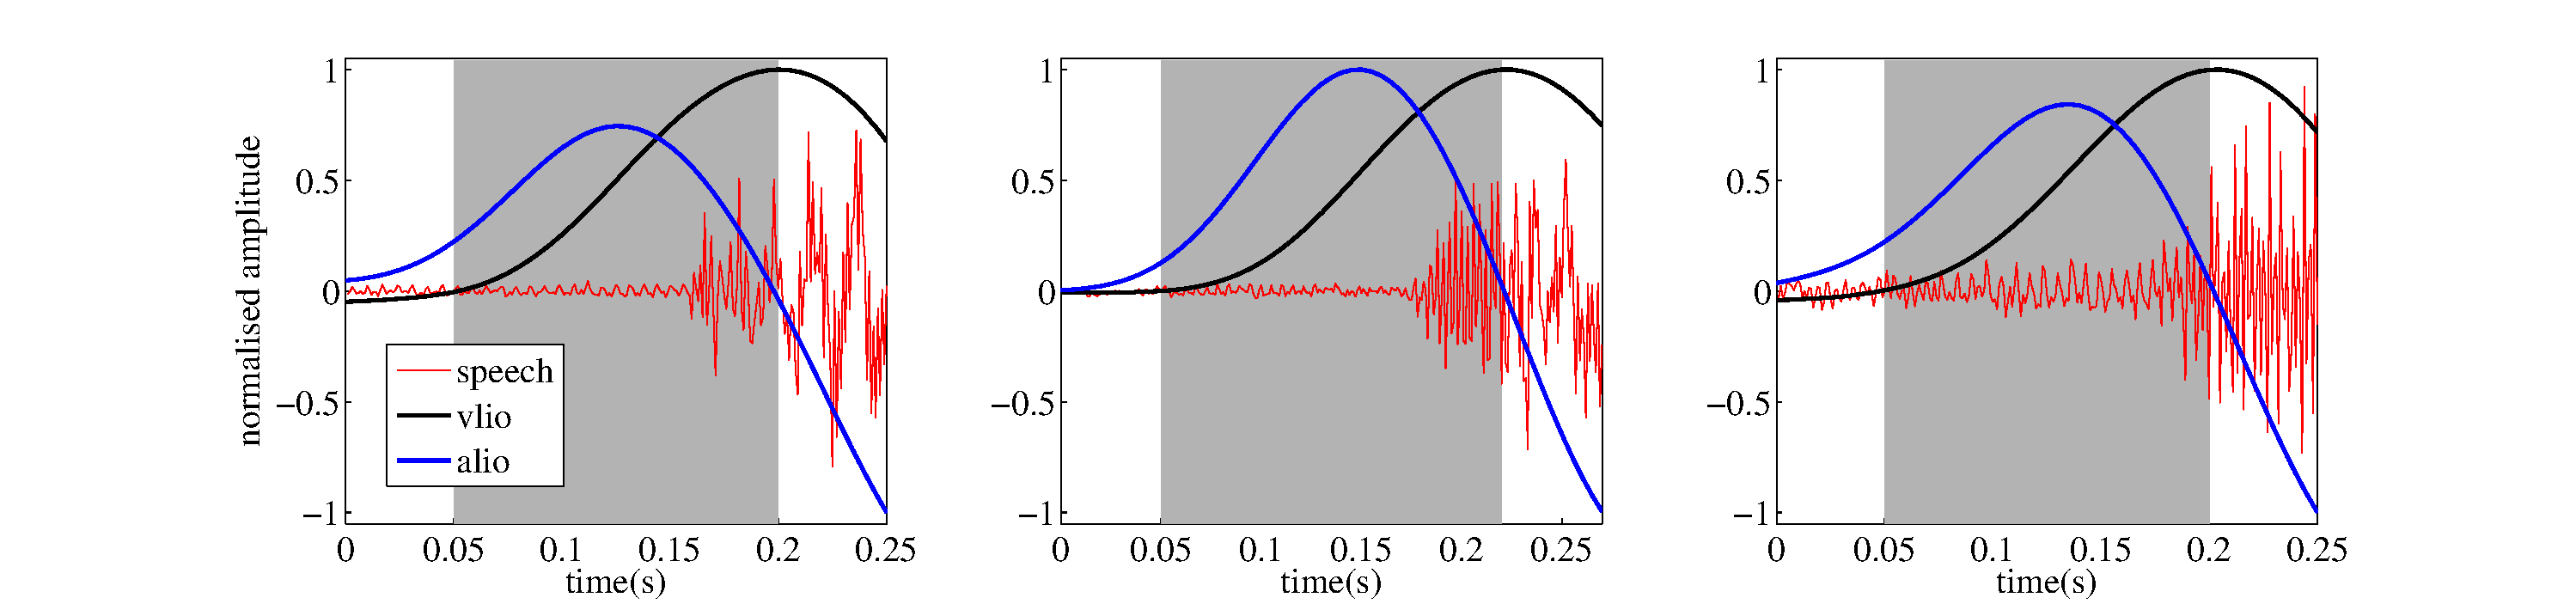
\includegraphics[width=4in]{figs/samples.eps}
\end{center}
\caption{{\bf Speech signal and motor trajectories.}The speech signal and motor trajectories 
(smoothed using a moving average filter) of lips opening
velocity (\vlio) and acceleration (\alio) during utterances containing /b/.
Left to right: /ba/, subject $5$; /ba/, subject $2$; and /bufalo/, subject $5$.
The gray zone denotes the detected start and ending of the plosion. All signals
are normalized over the indicated time frame, for visualization purposes.}
\label{fig:isdView}
\end{figure}

\begin{figure}[t]
\begin{center}
%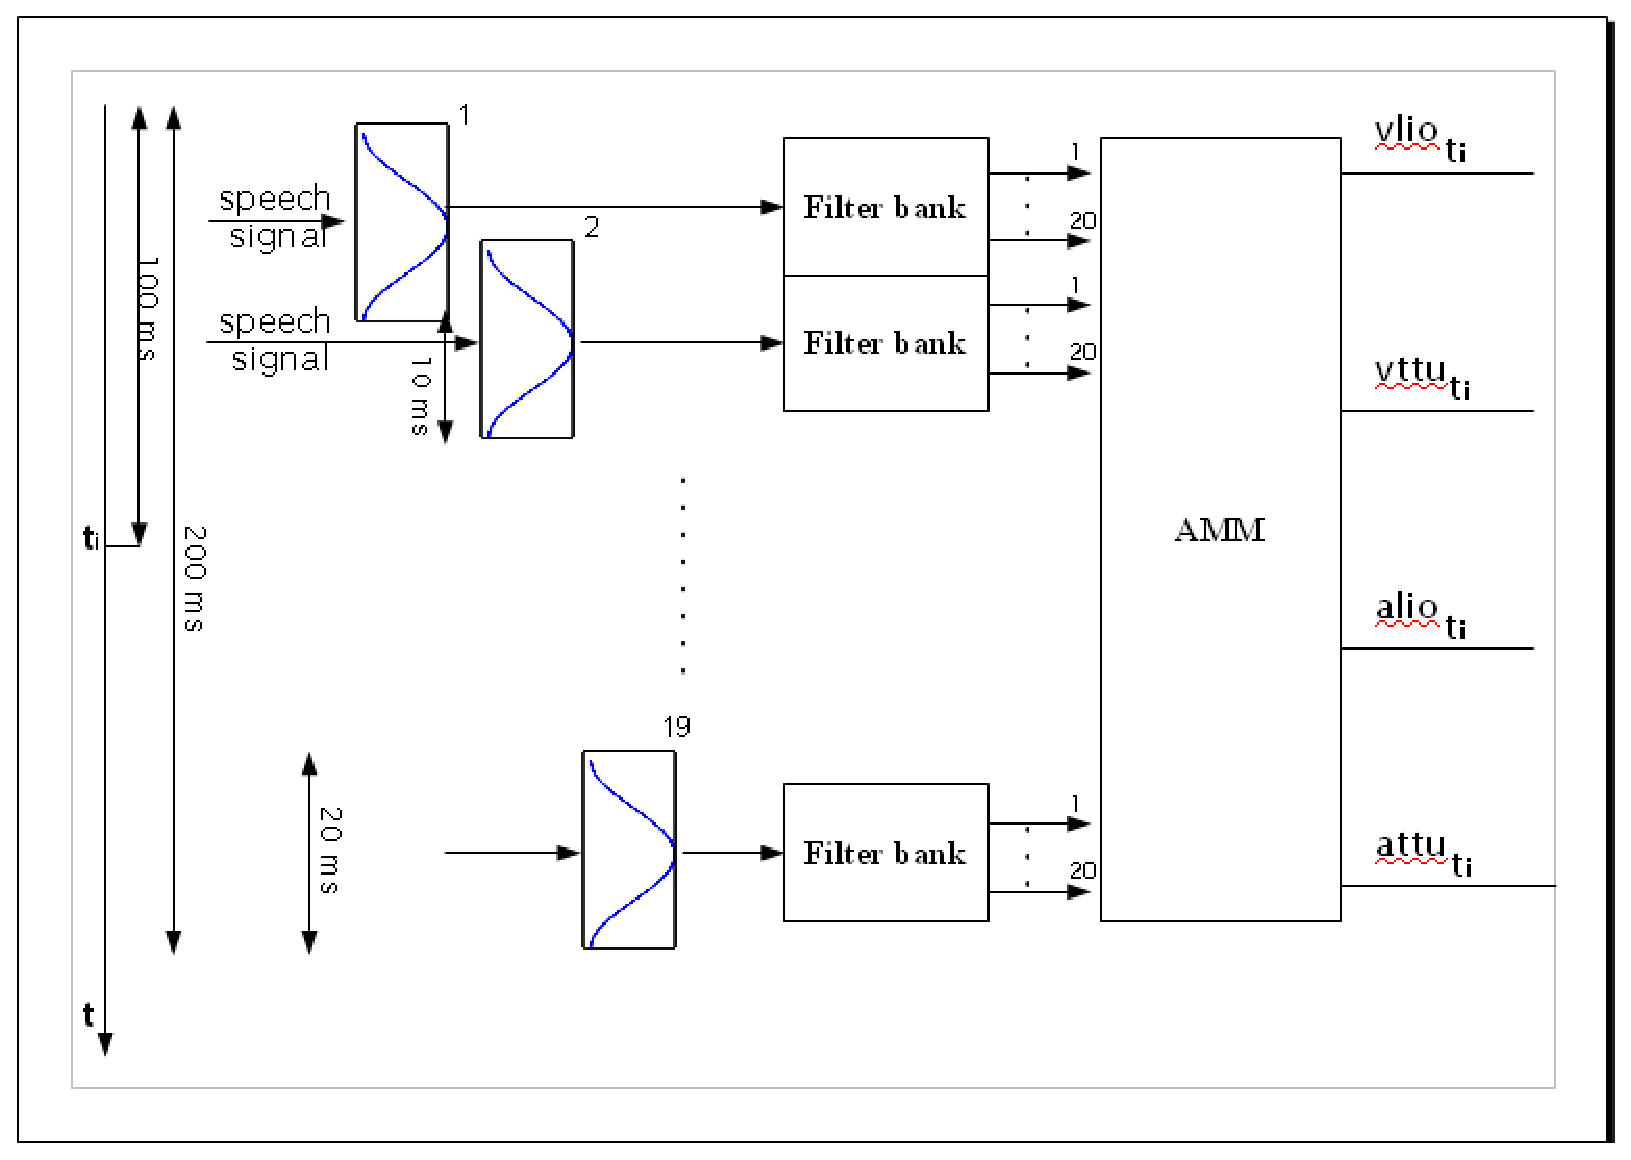
\includegraphics[width=4in]{figs/audio2motor.eps}
\end{center}
\caption{{\bf From speech signal to reconstructed motor information.} The AMM is first trained on training speech data and then used, during testing, to reconstruct motor information from the testing speech data. To reconstruct a single sample of \vlio, \alio, \vttu\ and \attu\ at time $t_i$ the
spectrogram of nineteen $20$-millisecond long Hamming windows is evaluated.
One window is centered at time $t_i$, $9$ windows precede it
and $9$ windows follow it. Each window overlaps by $10$ milliseconds
with the preceding window. The spectrogram is computed by using a
$20$-filter Mel-scale filterbank.}
\label{fig:amm}
\end{figure}

\begin{figure}[ht]
\begin{center}
%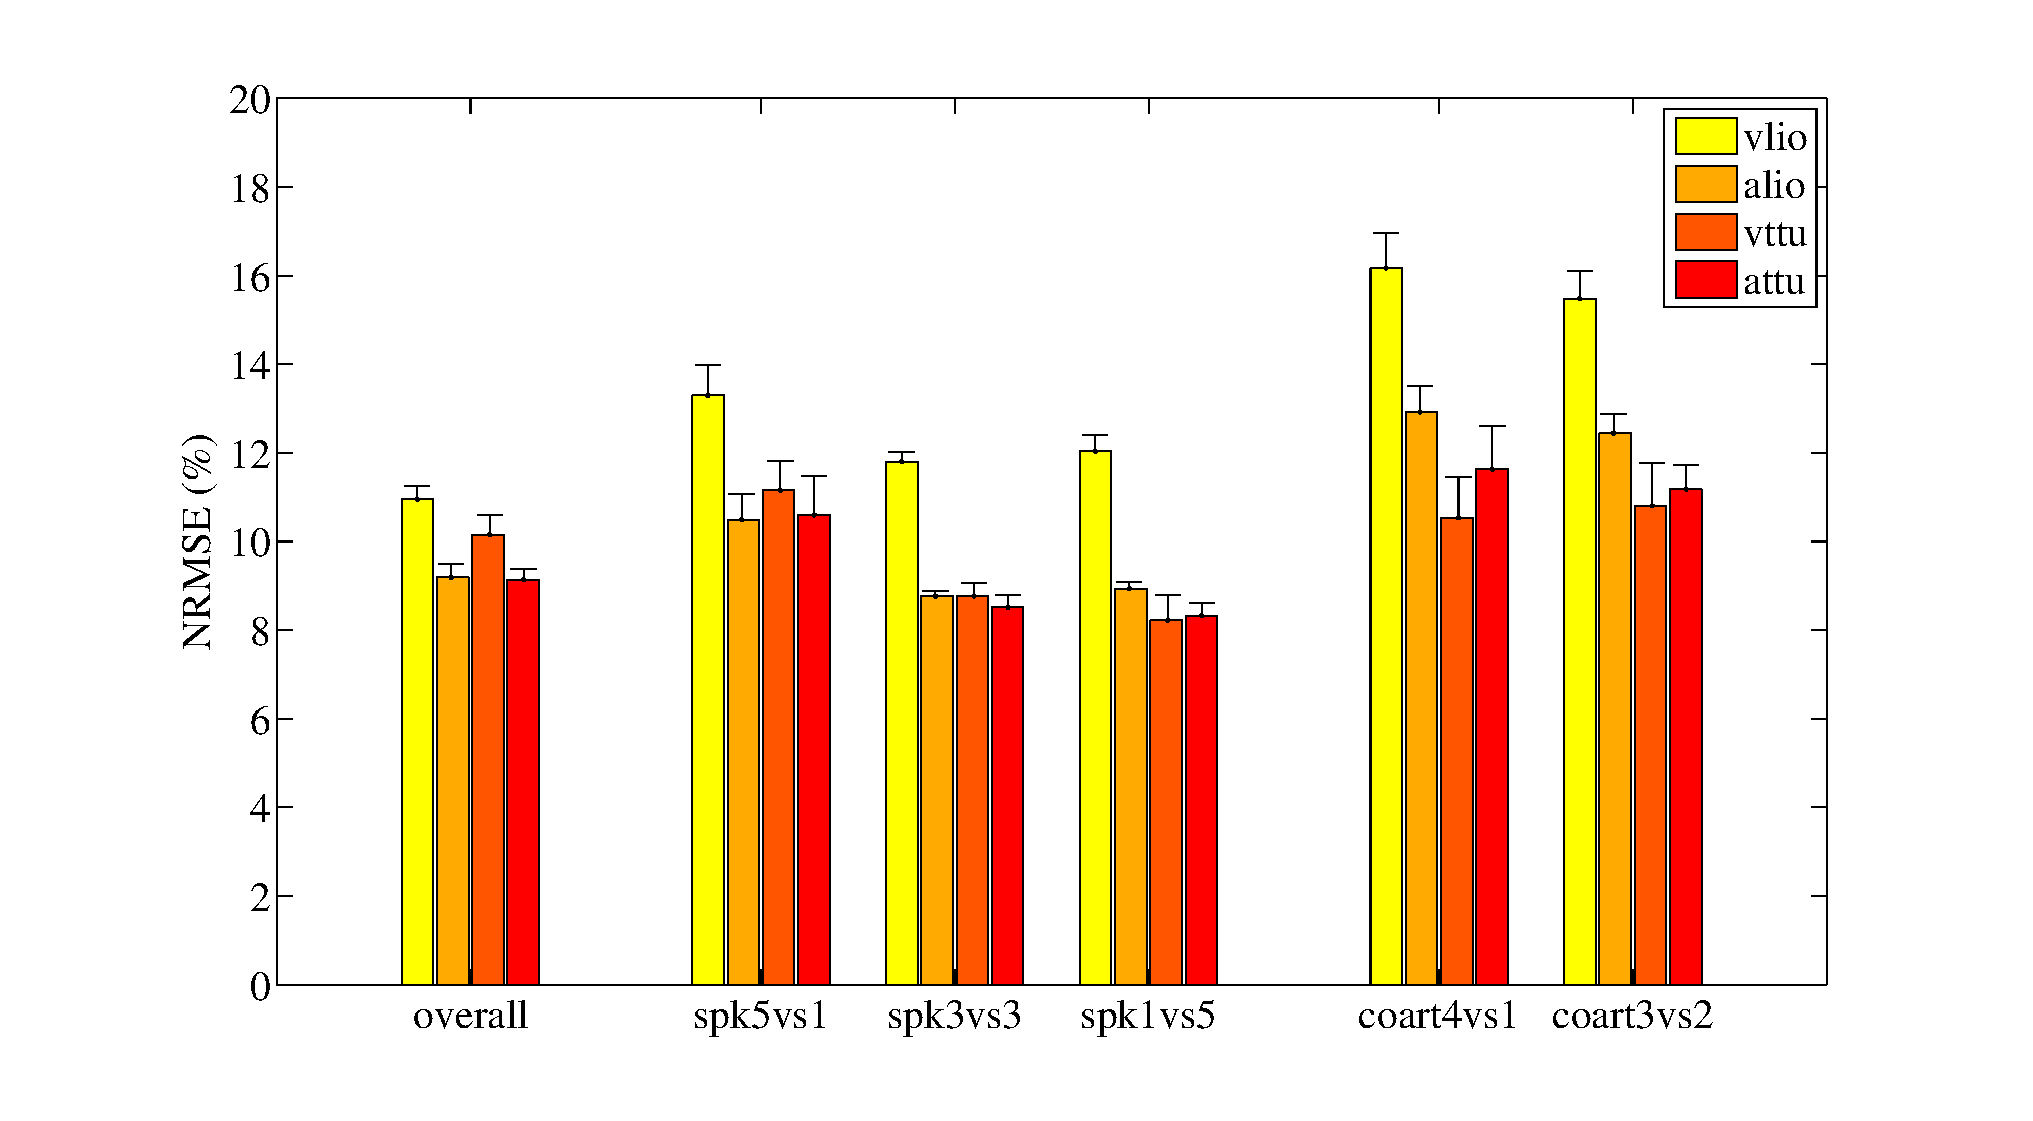
\includegraphics[width=4in]{figs/AMM.eps}
\end{center} 
\caption{{\bf Quantitative performance of the AMM.} For each cross-validation schema (overall, etc.)
and output signal (\vlio, etc.) the NRMSE average value and standard error of the mean
are reported.} \label{fig:amm_perf}
\end{figure}

\begin{figure}[t]
%\centerline{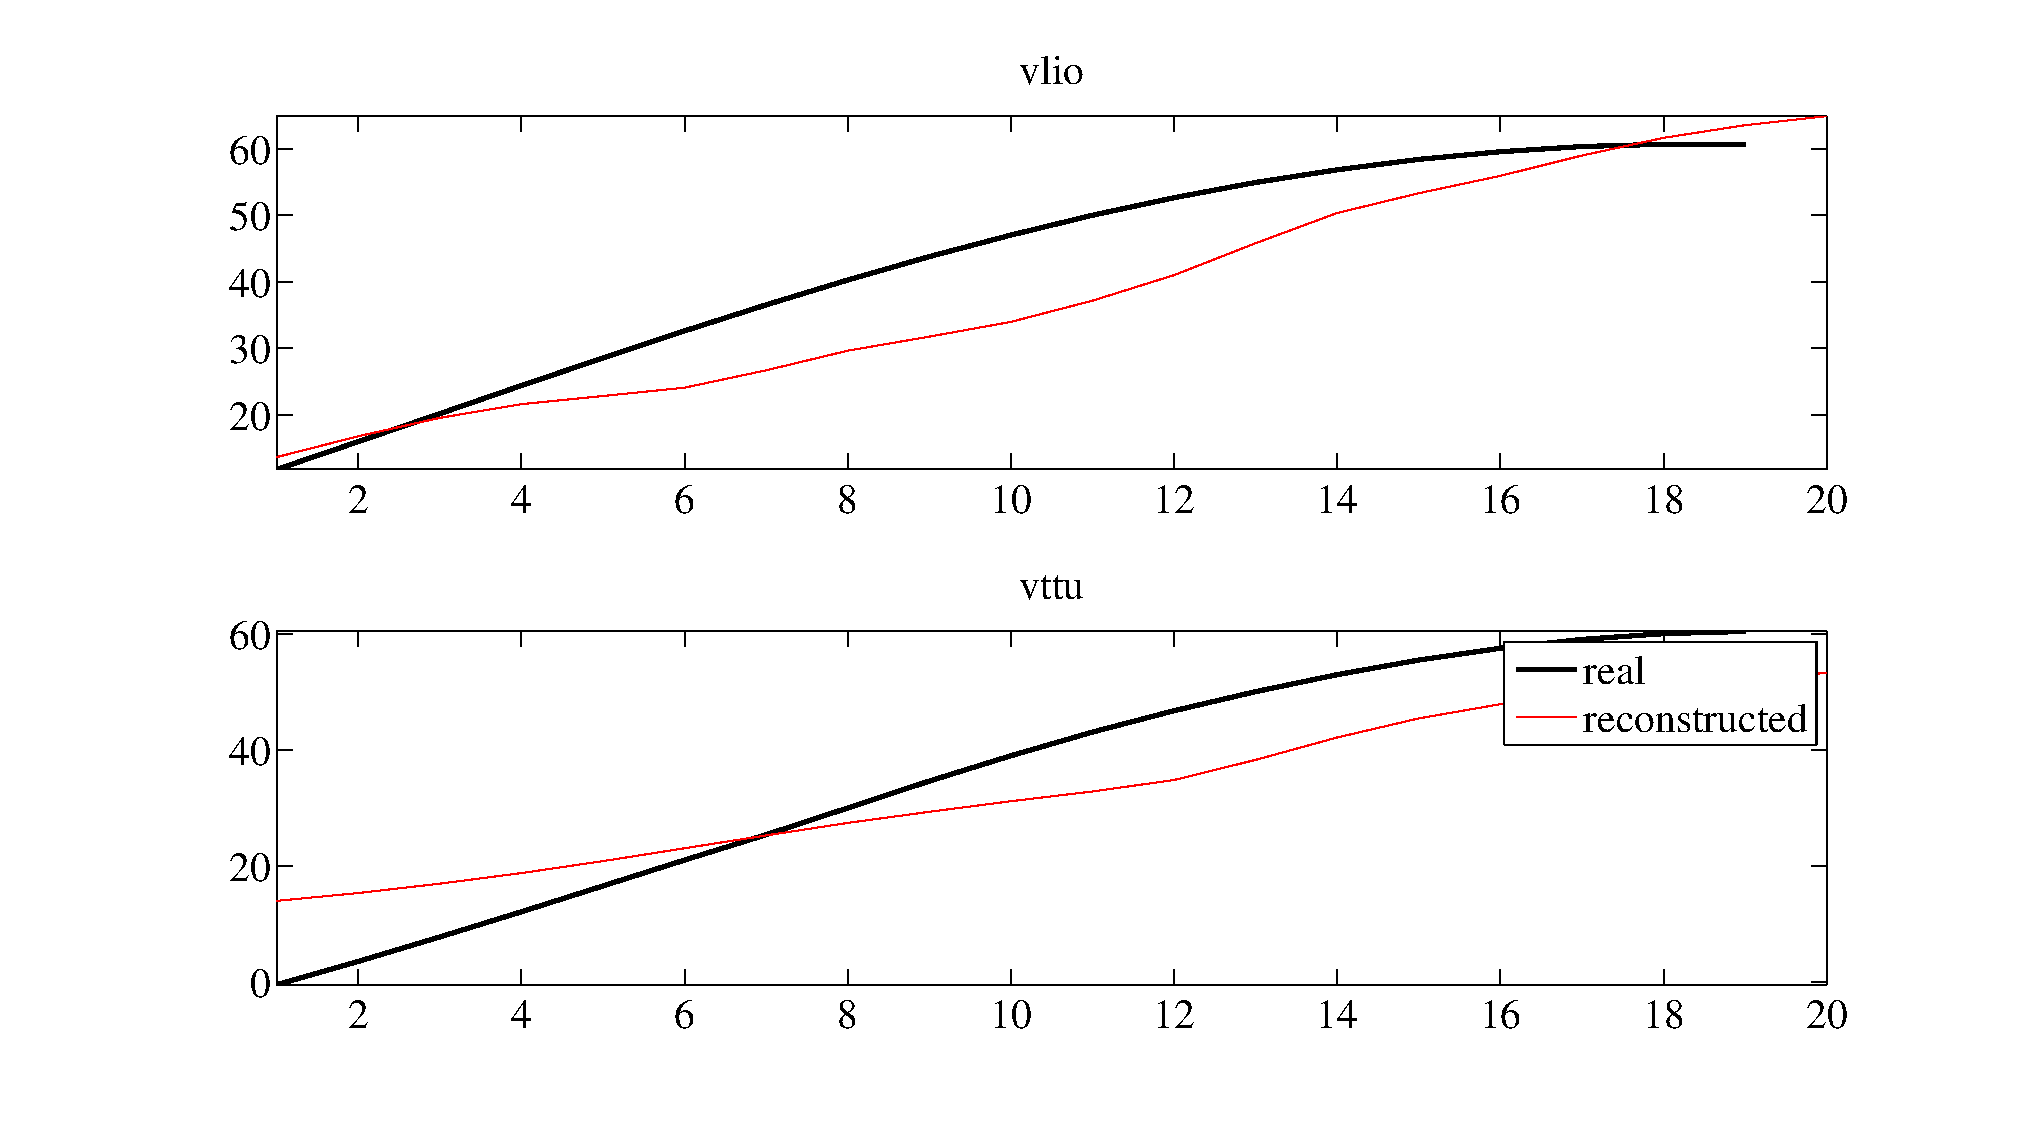
\includegraphics[width=4in]{figs/recMIs.eps}}
\caption{{\bf Real and AMM-reconstructed motor features.} Real and AMM-reconstructed \vlio\ and \vttu\ for subject $6$ uttering
the /t/ in \emph{accento?} (accent). Notice the apparent gap in the quality
of the reconstruction, favoring in this case the labiodental trajectory (\vttu).}
\label{fig:example}
\end{figure}

\begin{figure}[t]
%\centerline{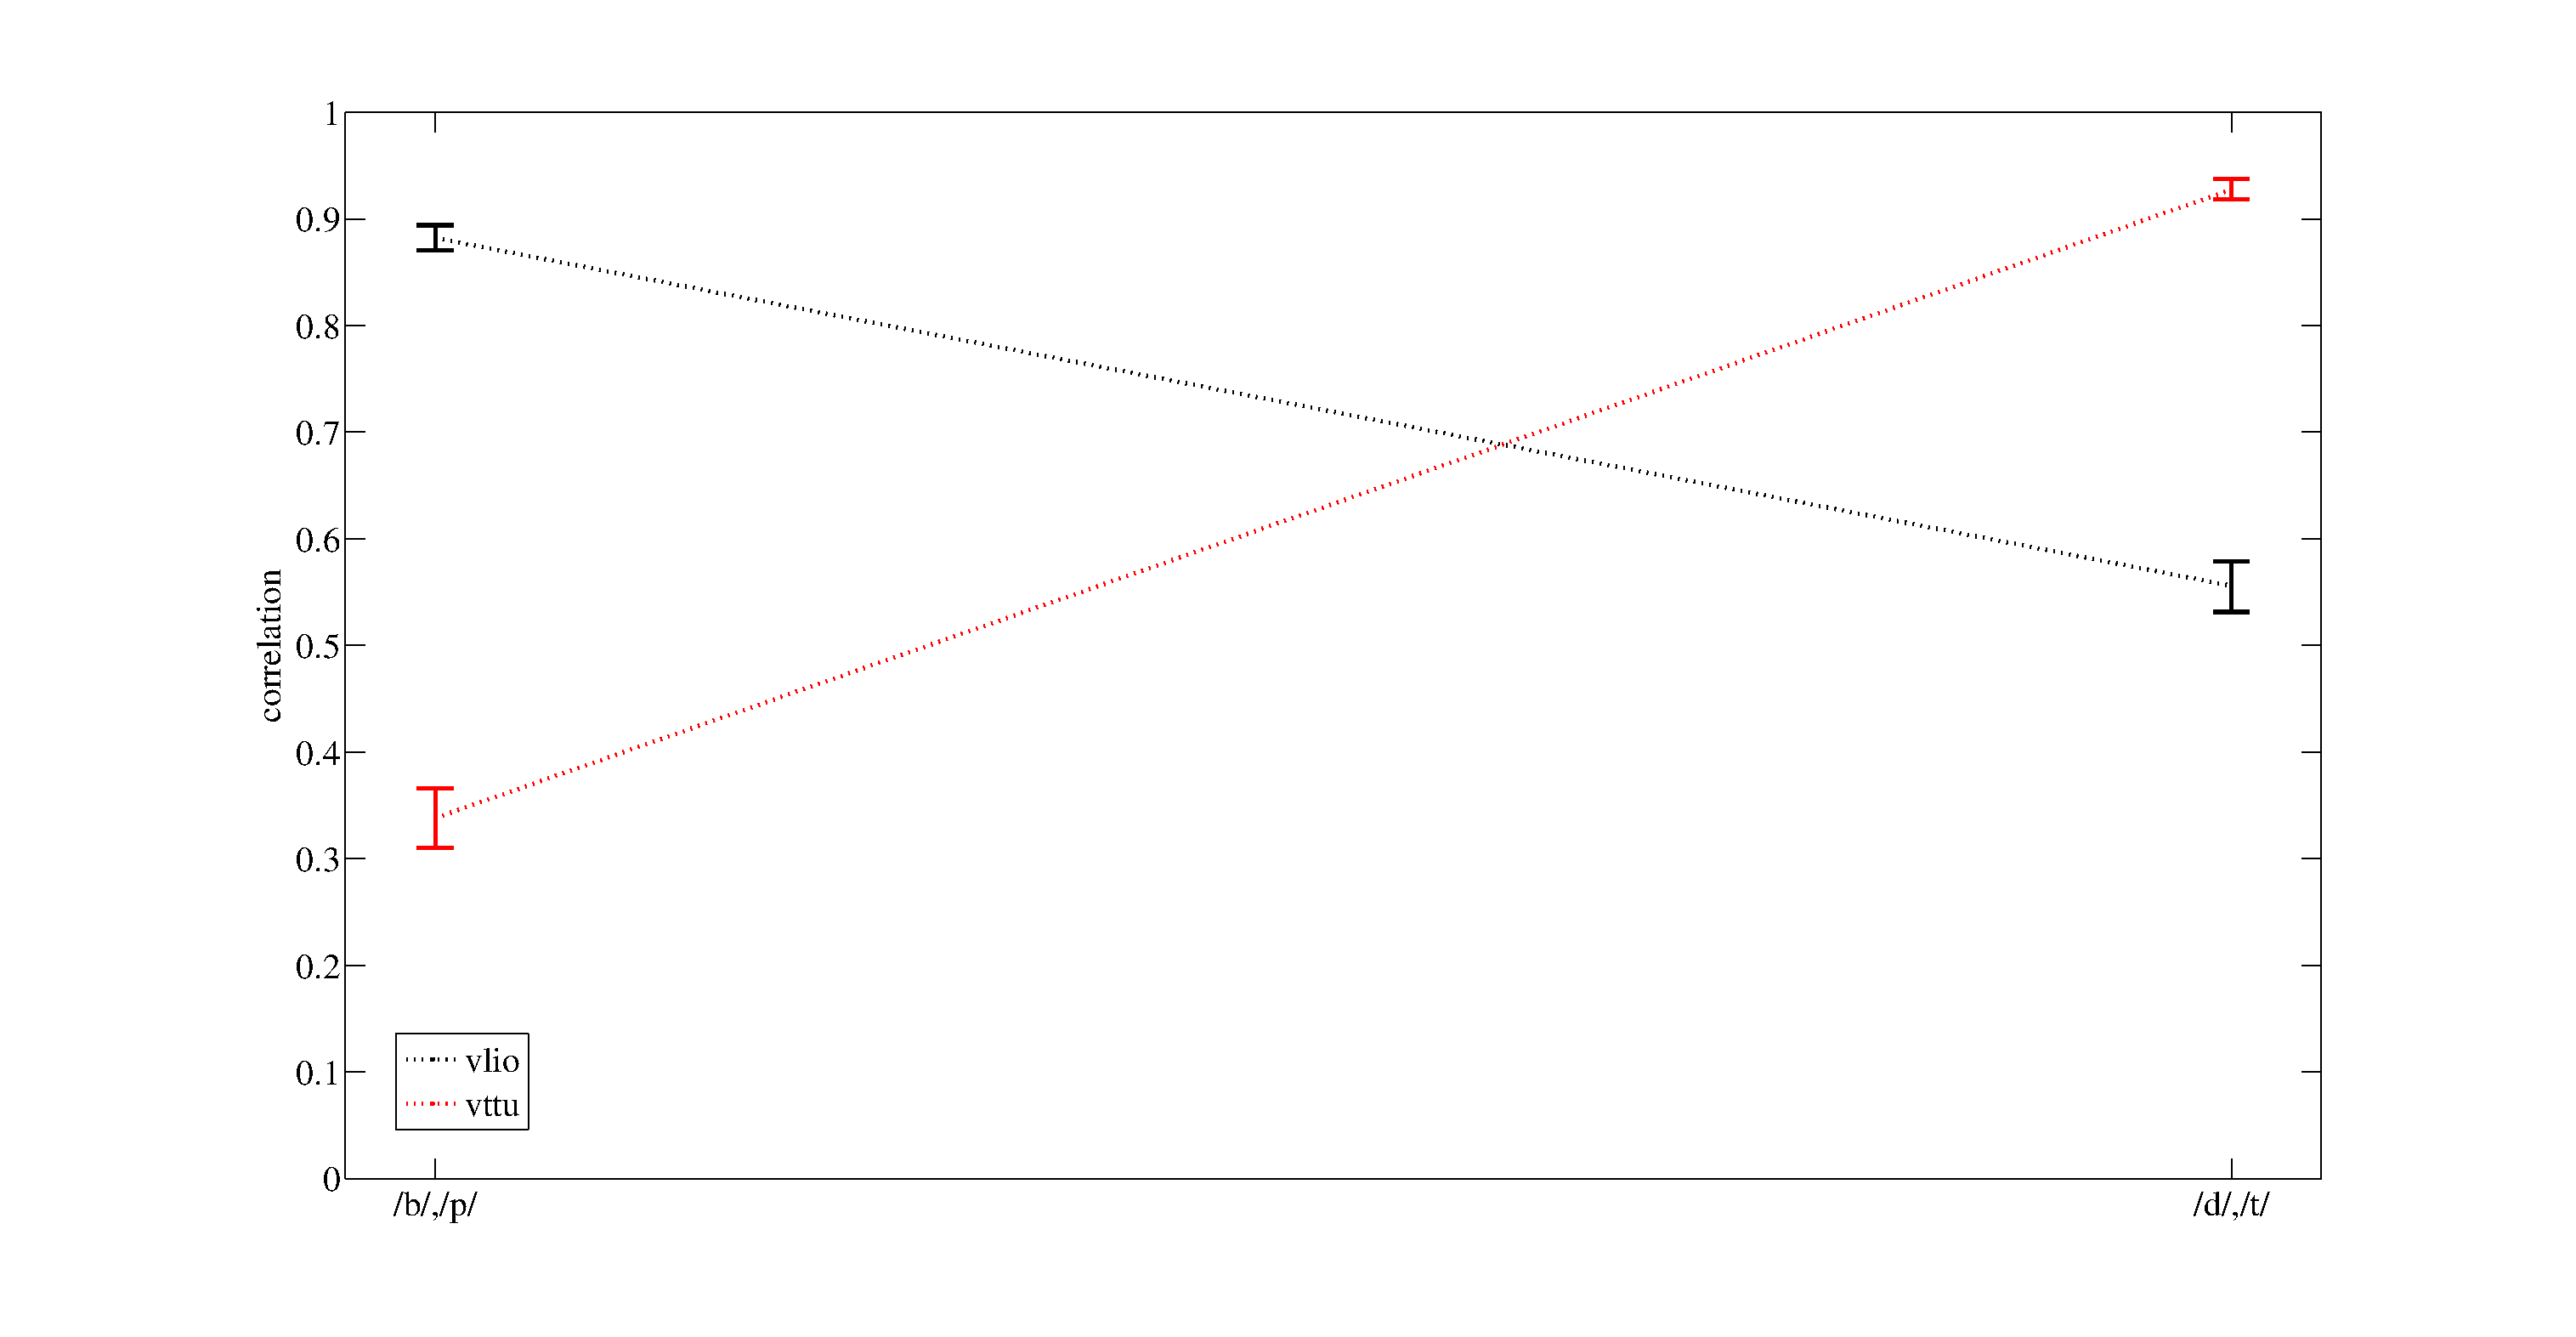
\includegraphics[width=4in]{figs/doubleDiss.eps}}
\caption{{\bf Double dissociation.} Double dissociation of correlation between real and AMM-reconstructed MI
(mean and standard error of the mean). Mean coefficients are significantly
higher for \vlio\ when ``listening'' to labials than dentals and vice-versa.
The \overall\ CV schema is used.}
\label{fig:DD}
\end{figure}

\begin{figure}[ht]
\begin{center}
%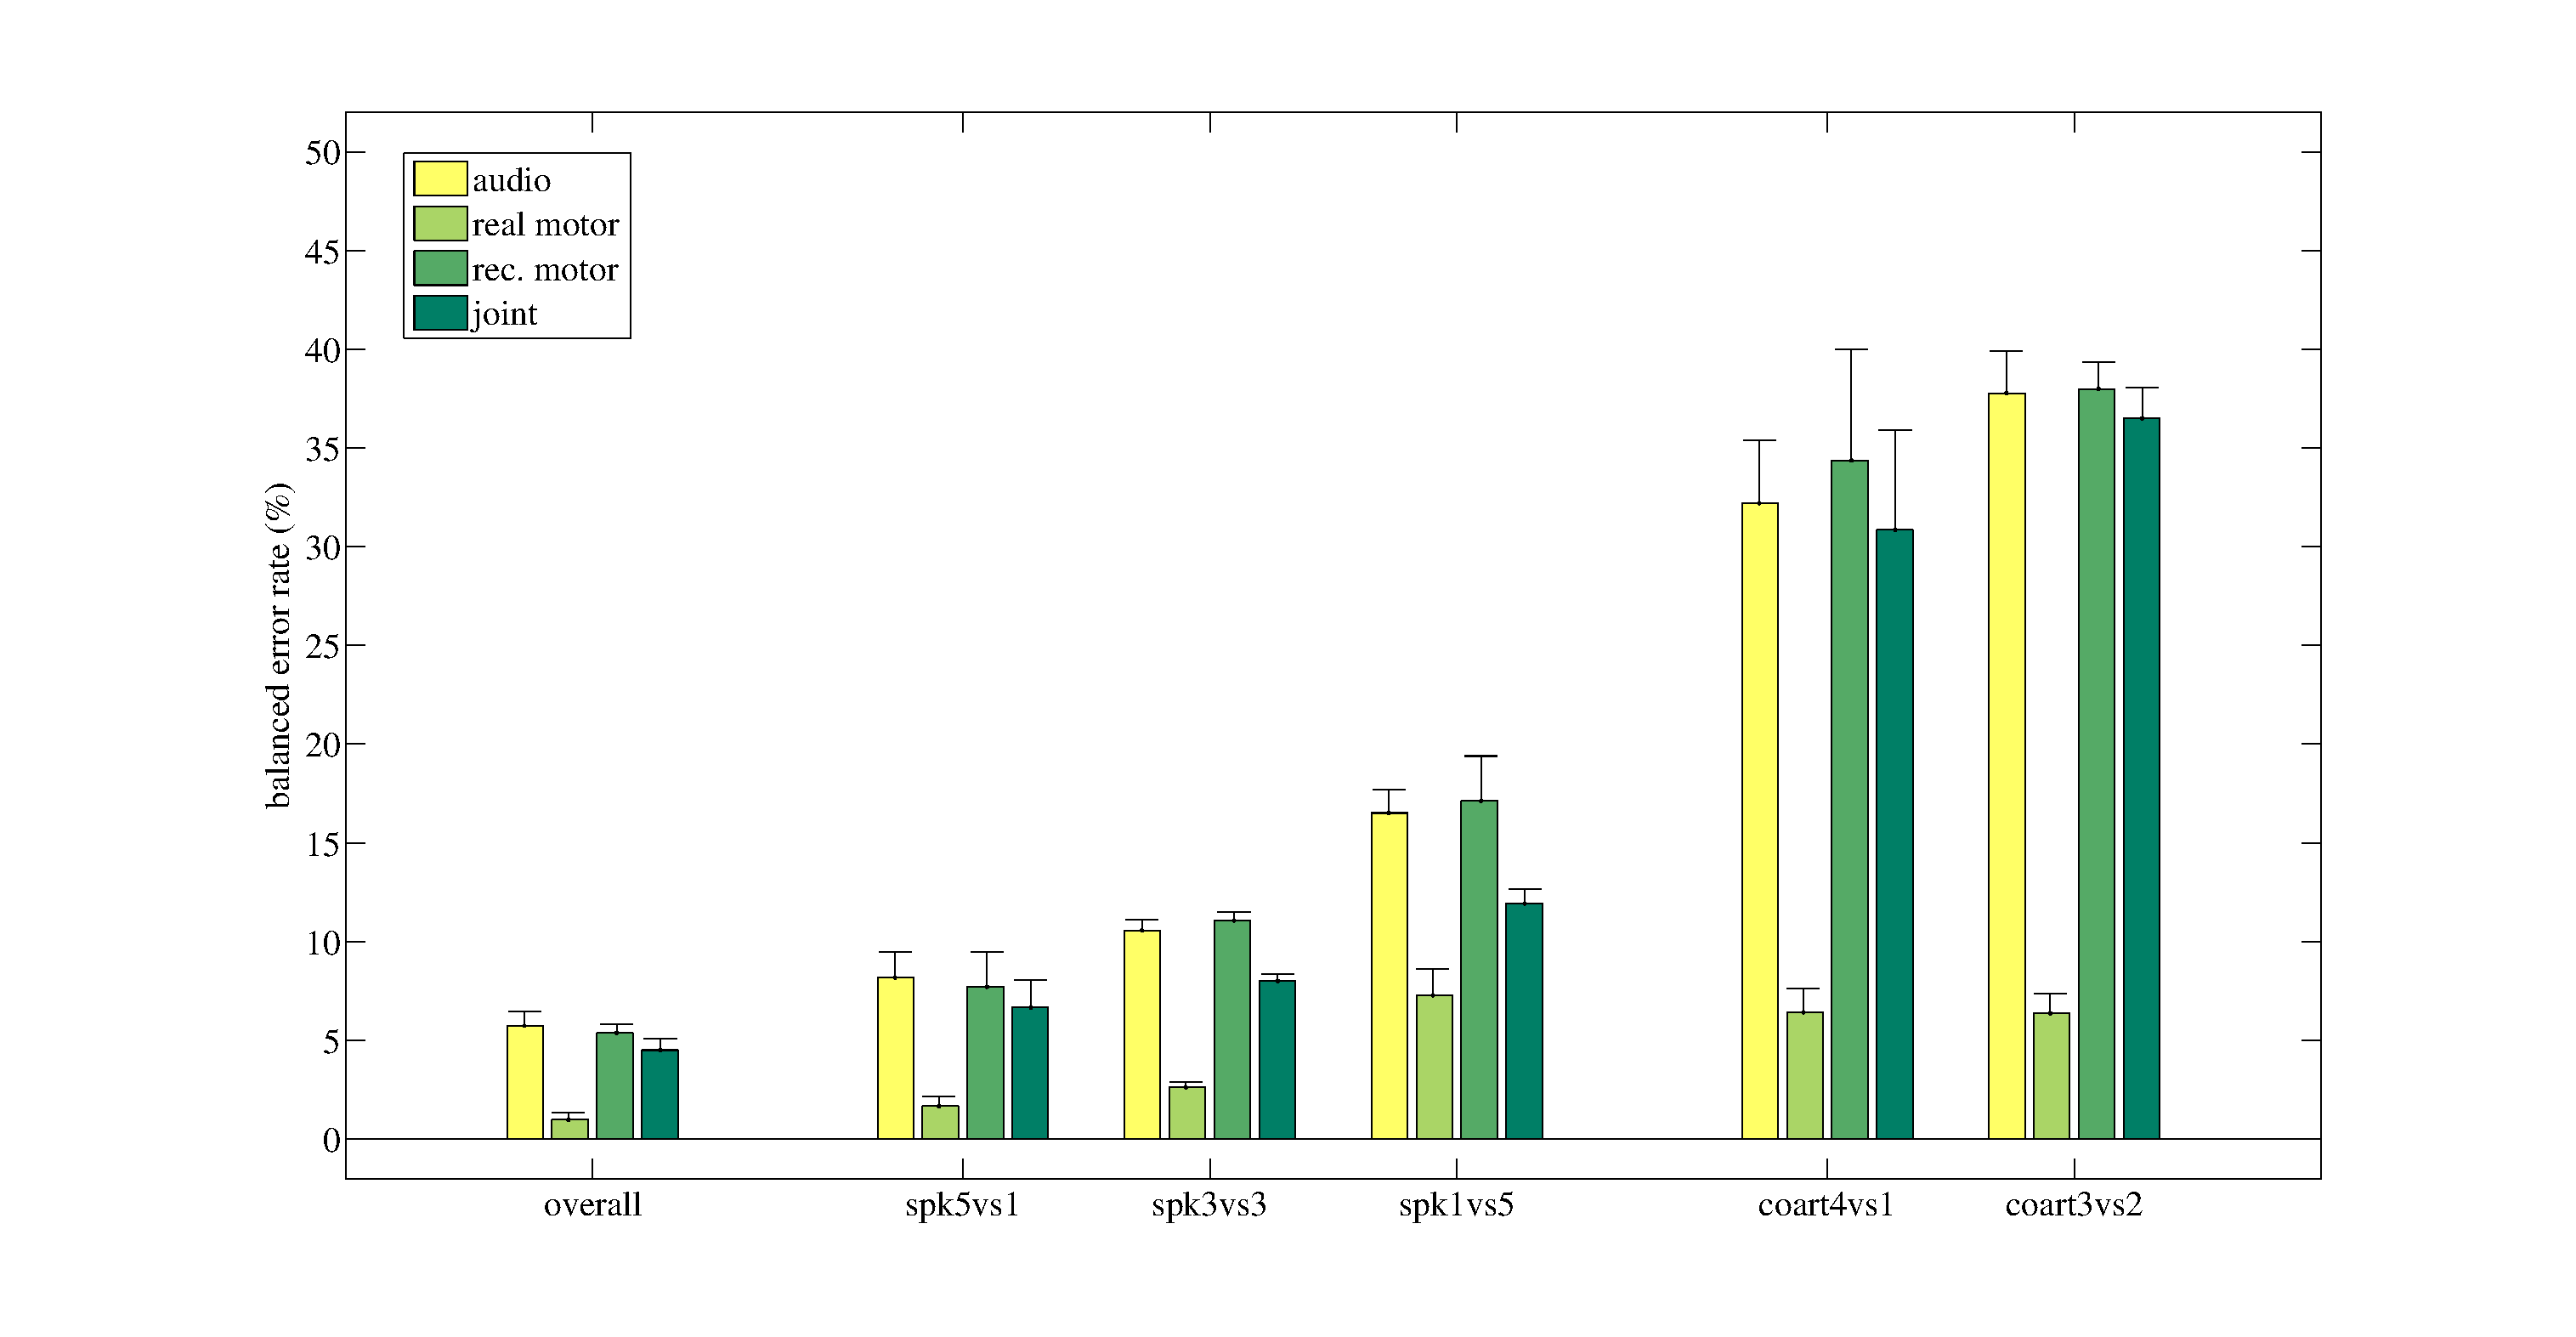
\includegraphics[width=4in]{figs/exp2.eps}
\end{center} 
\caption{ {\bf Results of experiment 1 and 2.} Balanced error rate in classification of bilabials and dentals for each
CV schema.}
\label{fig:class2_perf}
% CV schema, using the four sets of features of Figure \ref{fig:class1_perf}.}
\end{figure}

\begin{figure}[ht]
\begin{center}
%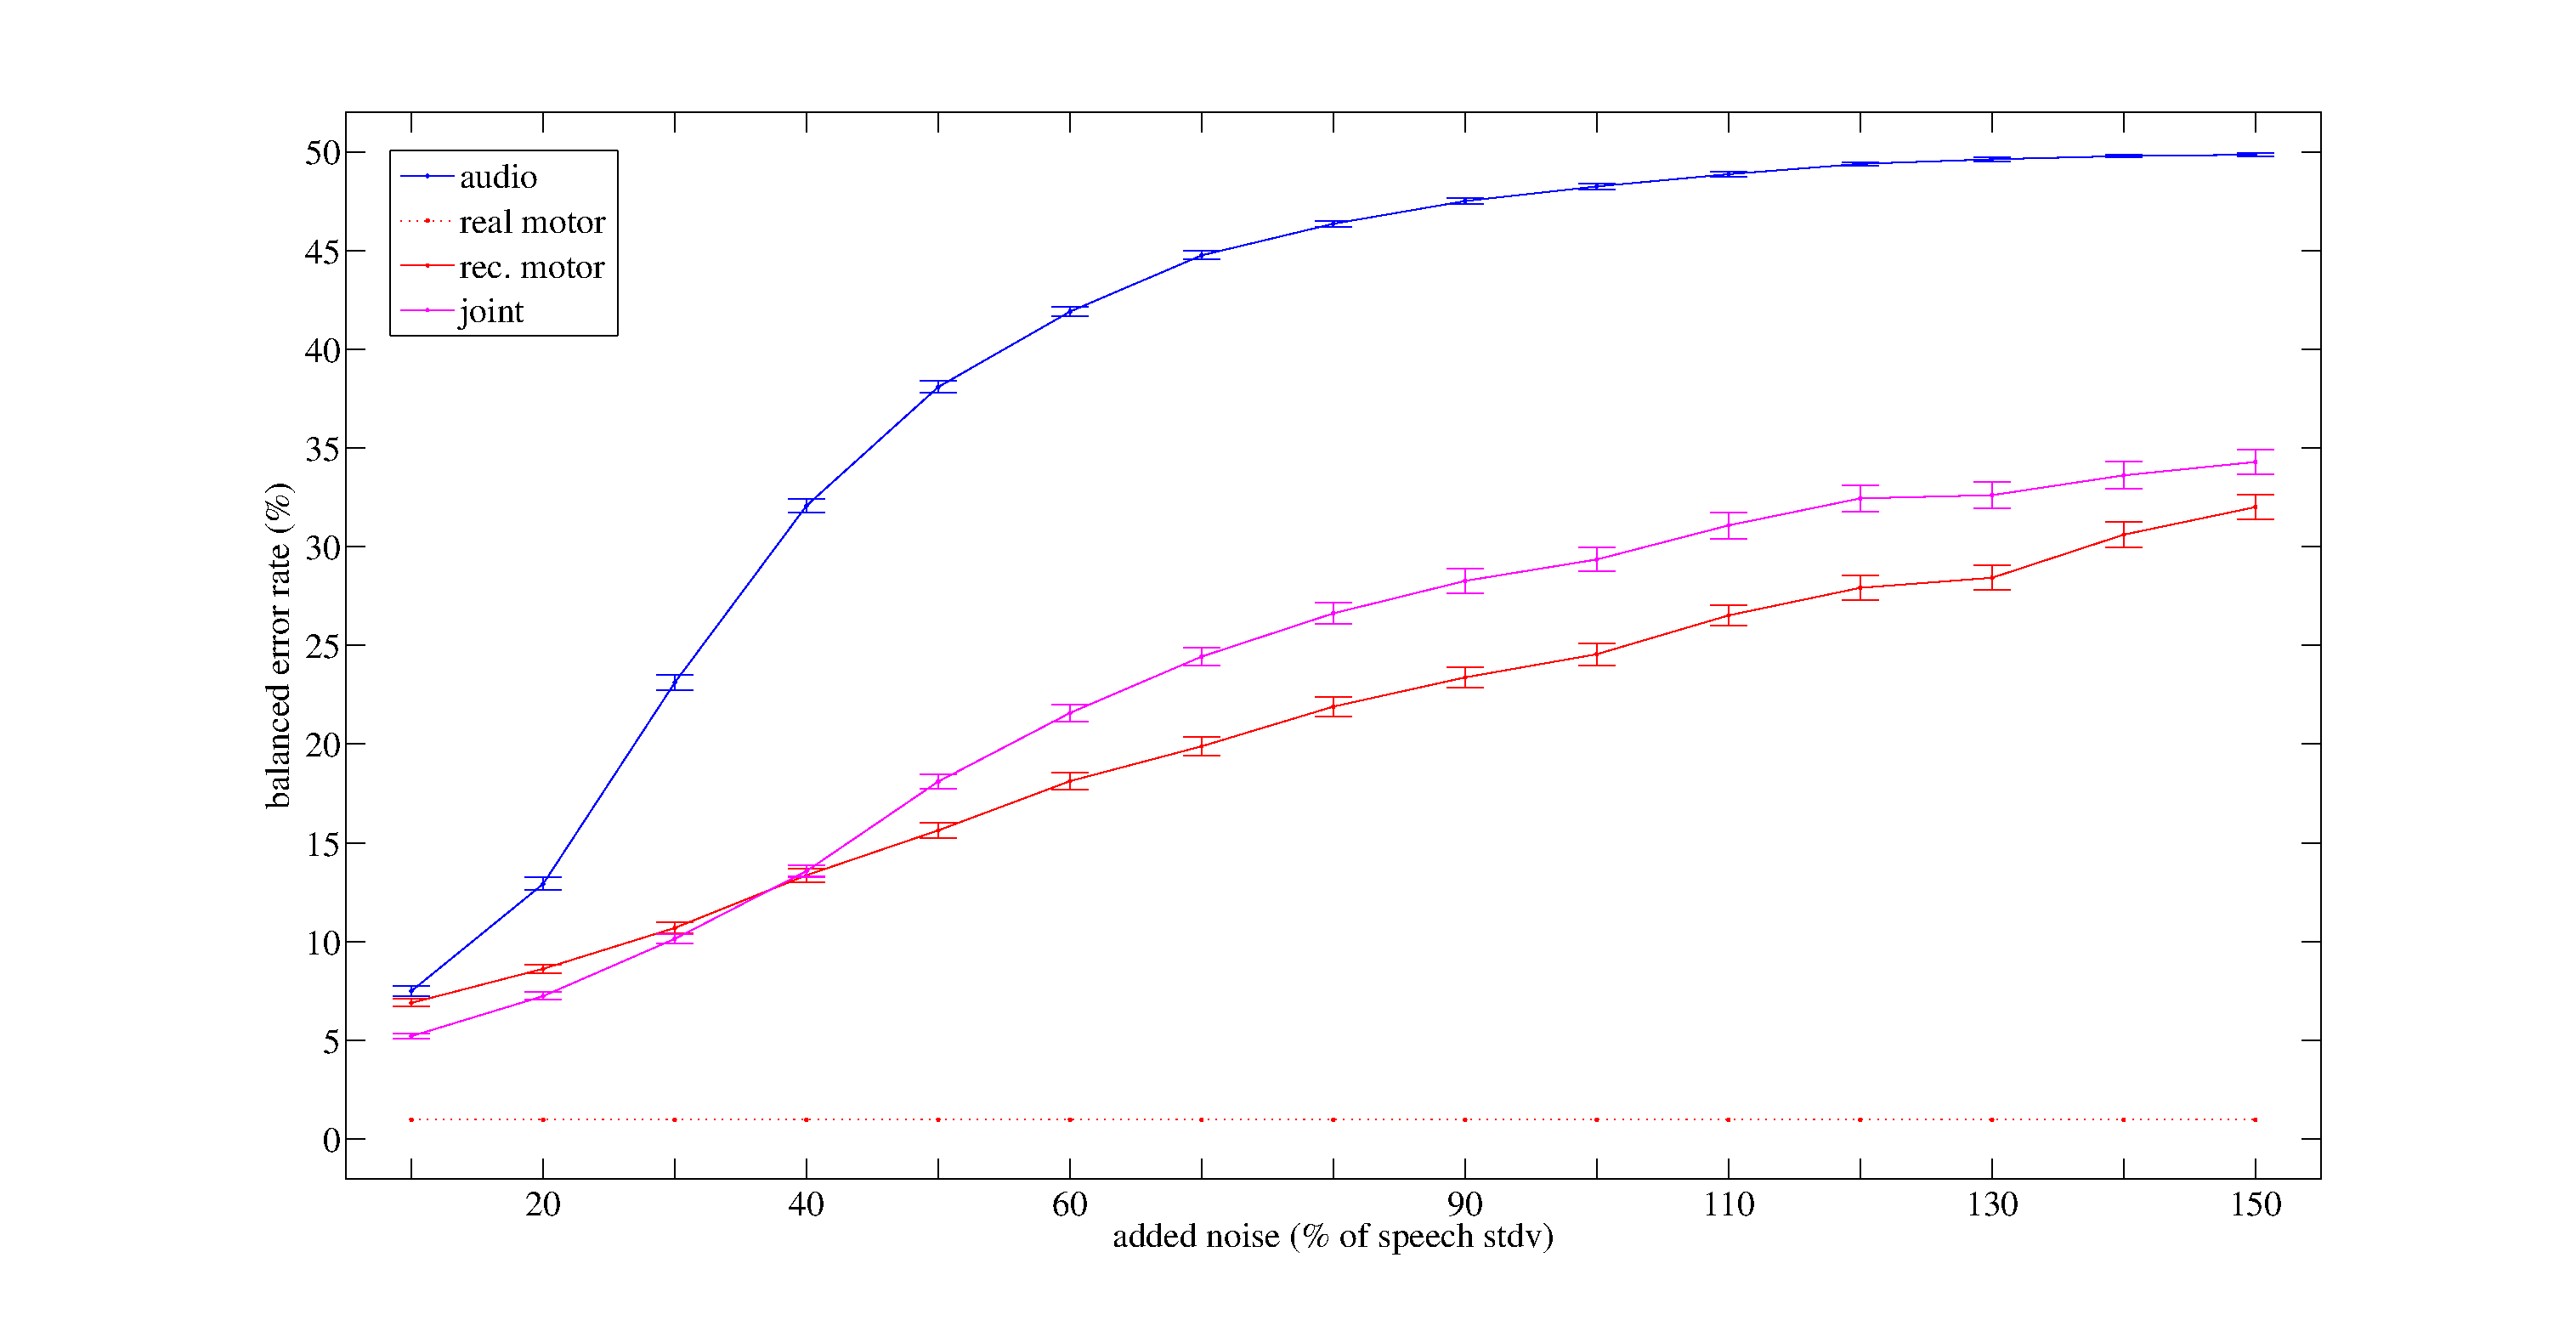
\includegraphics[width=4in]{figs/exp3.eps}
\end{center} 
\caption{{\bf Results of experiment 3.} Balanced error rate in classification of bilabials and dentals for the
\overall\ CV schema as noise is added.}
% \overall\ CV schema as noise is added, using the sets of features of Figure
% \ref{fig:class2_perf}.}
\label{fig:class3_perf}
\end{figure}


%\section*{Tables}
%\begin{table}[!ht]
%\caption{
%\bf{Table title}}
%\begin{tabular}{|c|c|c|}
%table information
%\end{tabular}
%\begin{flushleft}Table caption
%\end{flushleft}
%\label{tab:label}
% \end{table}

\end{document}

